\section{Scenario-based Two-stage Re-Optimization heuristic}
\label{subsection:proposed_method_generalization}

One of the main ideas behind rolling horizon methods, such as RI, is that a finite number of sampled scenarios can be used to approximate the sample space of a continuous-state problem. The RI heuristic has shown promising performance in various applications and is simple and intuitive. We utilize a similar concept as the RI heuristic in developing a novel Scenario-based Two-stage Re-Optimization heuristic (STRO). Instead of using expectations of exogenous variables as forecasts from any given state, we propose to generate possible scenarios from the stochastic model and repeatedly solve two-stage problems based on these scenarios.

To distinguish between the outer scenarios that are the realizations of the environment that are unknown to the heuristic, and the inner scenarios that are generated to build the two-stage stochastic programs that the heuristic solves to find the first-stage decision. We refer to the outer scenarios as level 1 scenarios and the inner ones as level 2 scenarios.

\color{red}
We introduce the following notation for formulating the two-stage problem used by the STRO scheme. Let $(I_t^{s},P_t^{s})$ denote the realization of stochastic variables in stage $t$ of level 1 scenario $s$. Let $l_t^{s}$ denote the endogenous stage reached at time $t$ by following the STRO scheme along level 1 scenario $s$. We denote the decision variables for discharge and spillage from reservoir $i$ in stage $t$ and level 1 scenario $s$ as $x_{i,t}^s$ and $r_{i,t}^n$ respectively. Furthermore, let $(\bar{\boldsymbol{I}}_t^{n},\bar{\boldsymbol{P}}_t^{n}) = \{(\bar{I}_t^{n},\bar{P}_t^{n}), (\bar{I}_{t+1}^{n},\bar{P}_{t+1}^{n}), ..., (\bar{I}_{T}^{n},\bar{P}_{T}^{n})\}$ denote a realization of level 2 scenario $n$ generated according to the stochastic processes, from time $t+1$ to end of horizon $T$, conditional on the level 1 realization at time $t$. Further, let the variables $\bar{l}_{i,t}^{n}, \bar{x}_{i,t}^{n}, \bar{r}_{i,t}^{n}$ represent the decision variables for the endogenous state, water discharge and spill for reservoir $i$ at time $t$ in level 2 scenario $n$. Let $\mathcal{T}_t = \{t, t+1, ..., T\}$ be the set of remaining periods from time $t$ to time $T$. For each stage $t$ and each level 1 scenario $s$, the two-stage problem that is being solved can be formulated as

\begin{equation}
\label{eq:twostage_formulation}
\begin{split}
    &\max_{\{(\boldsymbol{\bar{l}}_\tau^n,\boldsymbol{\bar{x}}_\tau^n,\boldsymbol{\bar{lr}}_\tau^n), n \in \mathcal{N}, \tau \in \mathcal{T}_t\}} \frac{1}{N} \sum_{n\in \mathcal{N}}\left( \sum_{\tau \in \mathcal{T}_t\setminus \{T\}}\beta^{\tau}\bar{P}^{n}_{\tau}\sum_{i\in R^P}g(\bar{l}_{i,\tau}^n,\bar{x}_{i,\tau}^n) + \beta^{T}\sum_{i\in R}\Phi_{i}(\bar{l}_{i,T}^n) \right), \\
    & \mathrm{s.t.} \ \ \ (l_{i,t}^s, P_{t}^s, I_{t}^s) = (\bar{l}_{i,t}^{n}, \bar{P}_t^{n}, \bar{I}_t^{n}), \quad \quad \quad \quad \quad \quad \quad \ \ n \in \mathcal{N}, i \in R \\
    & \quad \quad \ \bar{l}^n_{i,\tau+1} = \bar{l}^n_{i,\tau} + \bar{I}^{n}_{i,\tau} - \bar{r}^n_{i,\tau} - \bar{x}^n_{i,\tau} + \sum_{j\in R_{i}^{Spill}} \bar{r}^n_{j,\tau}+ \sum_{j\in R_{i}^{Dis}} \bar{x}^n_{j,\tau}, \quad \tau \in \mathcal{T}_t \setminus \{T\} \quad i\in R  \quad n\in \mathcal{N}\\
    & \quad \quad \ x^s_{i,t} =  \bar{x}^{n}_{i,t}, \quad \quad n \in \mathcal{N}, i\in R \\
    & \quad \quad \ r^s_{i,t} =  \bar{r}^{n}_{i,t}, \quad \quad n \in \mathcal{N}, i\in R 
\end{split}
\end{equation}
The objective of the two-stage problem is to maximize expected future profits in the discrete set of (level 2) scenarios $\mathcal{N}$. In this formulation, every scenario in $\mathcal{N}$ is considered equally likely, but it is also possible to introduce a separate weighting for each scenario if they have different likelihoods. The first constraint ensures that the initial condition is set to the realized time-$t$ level 1 scenario $s$ and the endogenous state reached in that scenario by following the STRO scheme. The next constraint is the reservoir balance in level 2 scenario $n$, which is equivalent to \eqref{eq:inventory_balance}. The last 2 constraints ensure that the first-stage decisions are the same in all level 2 scenarios $n \in \mathcal{N}$ and that the production decisions that will be used in level 1 scenario $s$ are the same as the first-stage decisions in the LP.  

Each time this problem is being solved, the time $t$ decisions, i.e. first-stage decisions, $(x_{i,t}^s, r_{i,t}^s)$ are used to update $l_{i,t}^s$ along the level 1 scenario $s$ according to equation \eqref{eq:inventory_balance}. This updated state then serves as an initial condition for the next two-stage problem. 

By generating $S$ level 1 scenarios, the total expected profits from the STRO scheme can be computed as the sample average
\begin{equation}
    \frac{1}{S} \sum_{s \in \mathcal{S}} \left( \sum_{t=0}^{T-1}\beta^{t}P^{s}_{t}\sum_{i\in R^P}g(l^{s}_{i,t},x^{s}_{i,t}) + \beta^{T}\sum_{i\in R}\Phi_{i}(l^{s}_{i,T}) \right)
\end{equation}

\color{black}
A visualization of how a two-stage stochastic program is built from generated level 2 scenarios to explore the underlying sample space can be seen in Figure \ref{fig:explorations stochastic program}. Starting in a state in stage $\tau$, one can generate $N$ possible realizations of the future, starting in the current state. Then, these scenarios can be combined into a two-stage stochastic program, which can be solved to find the first-stage decision.

\begin{figure}[H]
    \centering
    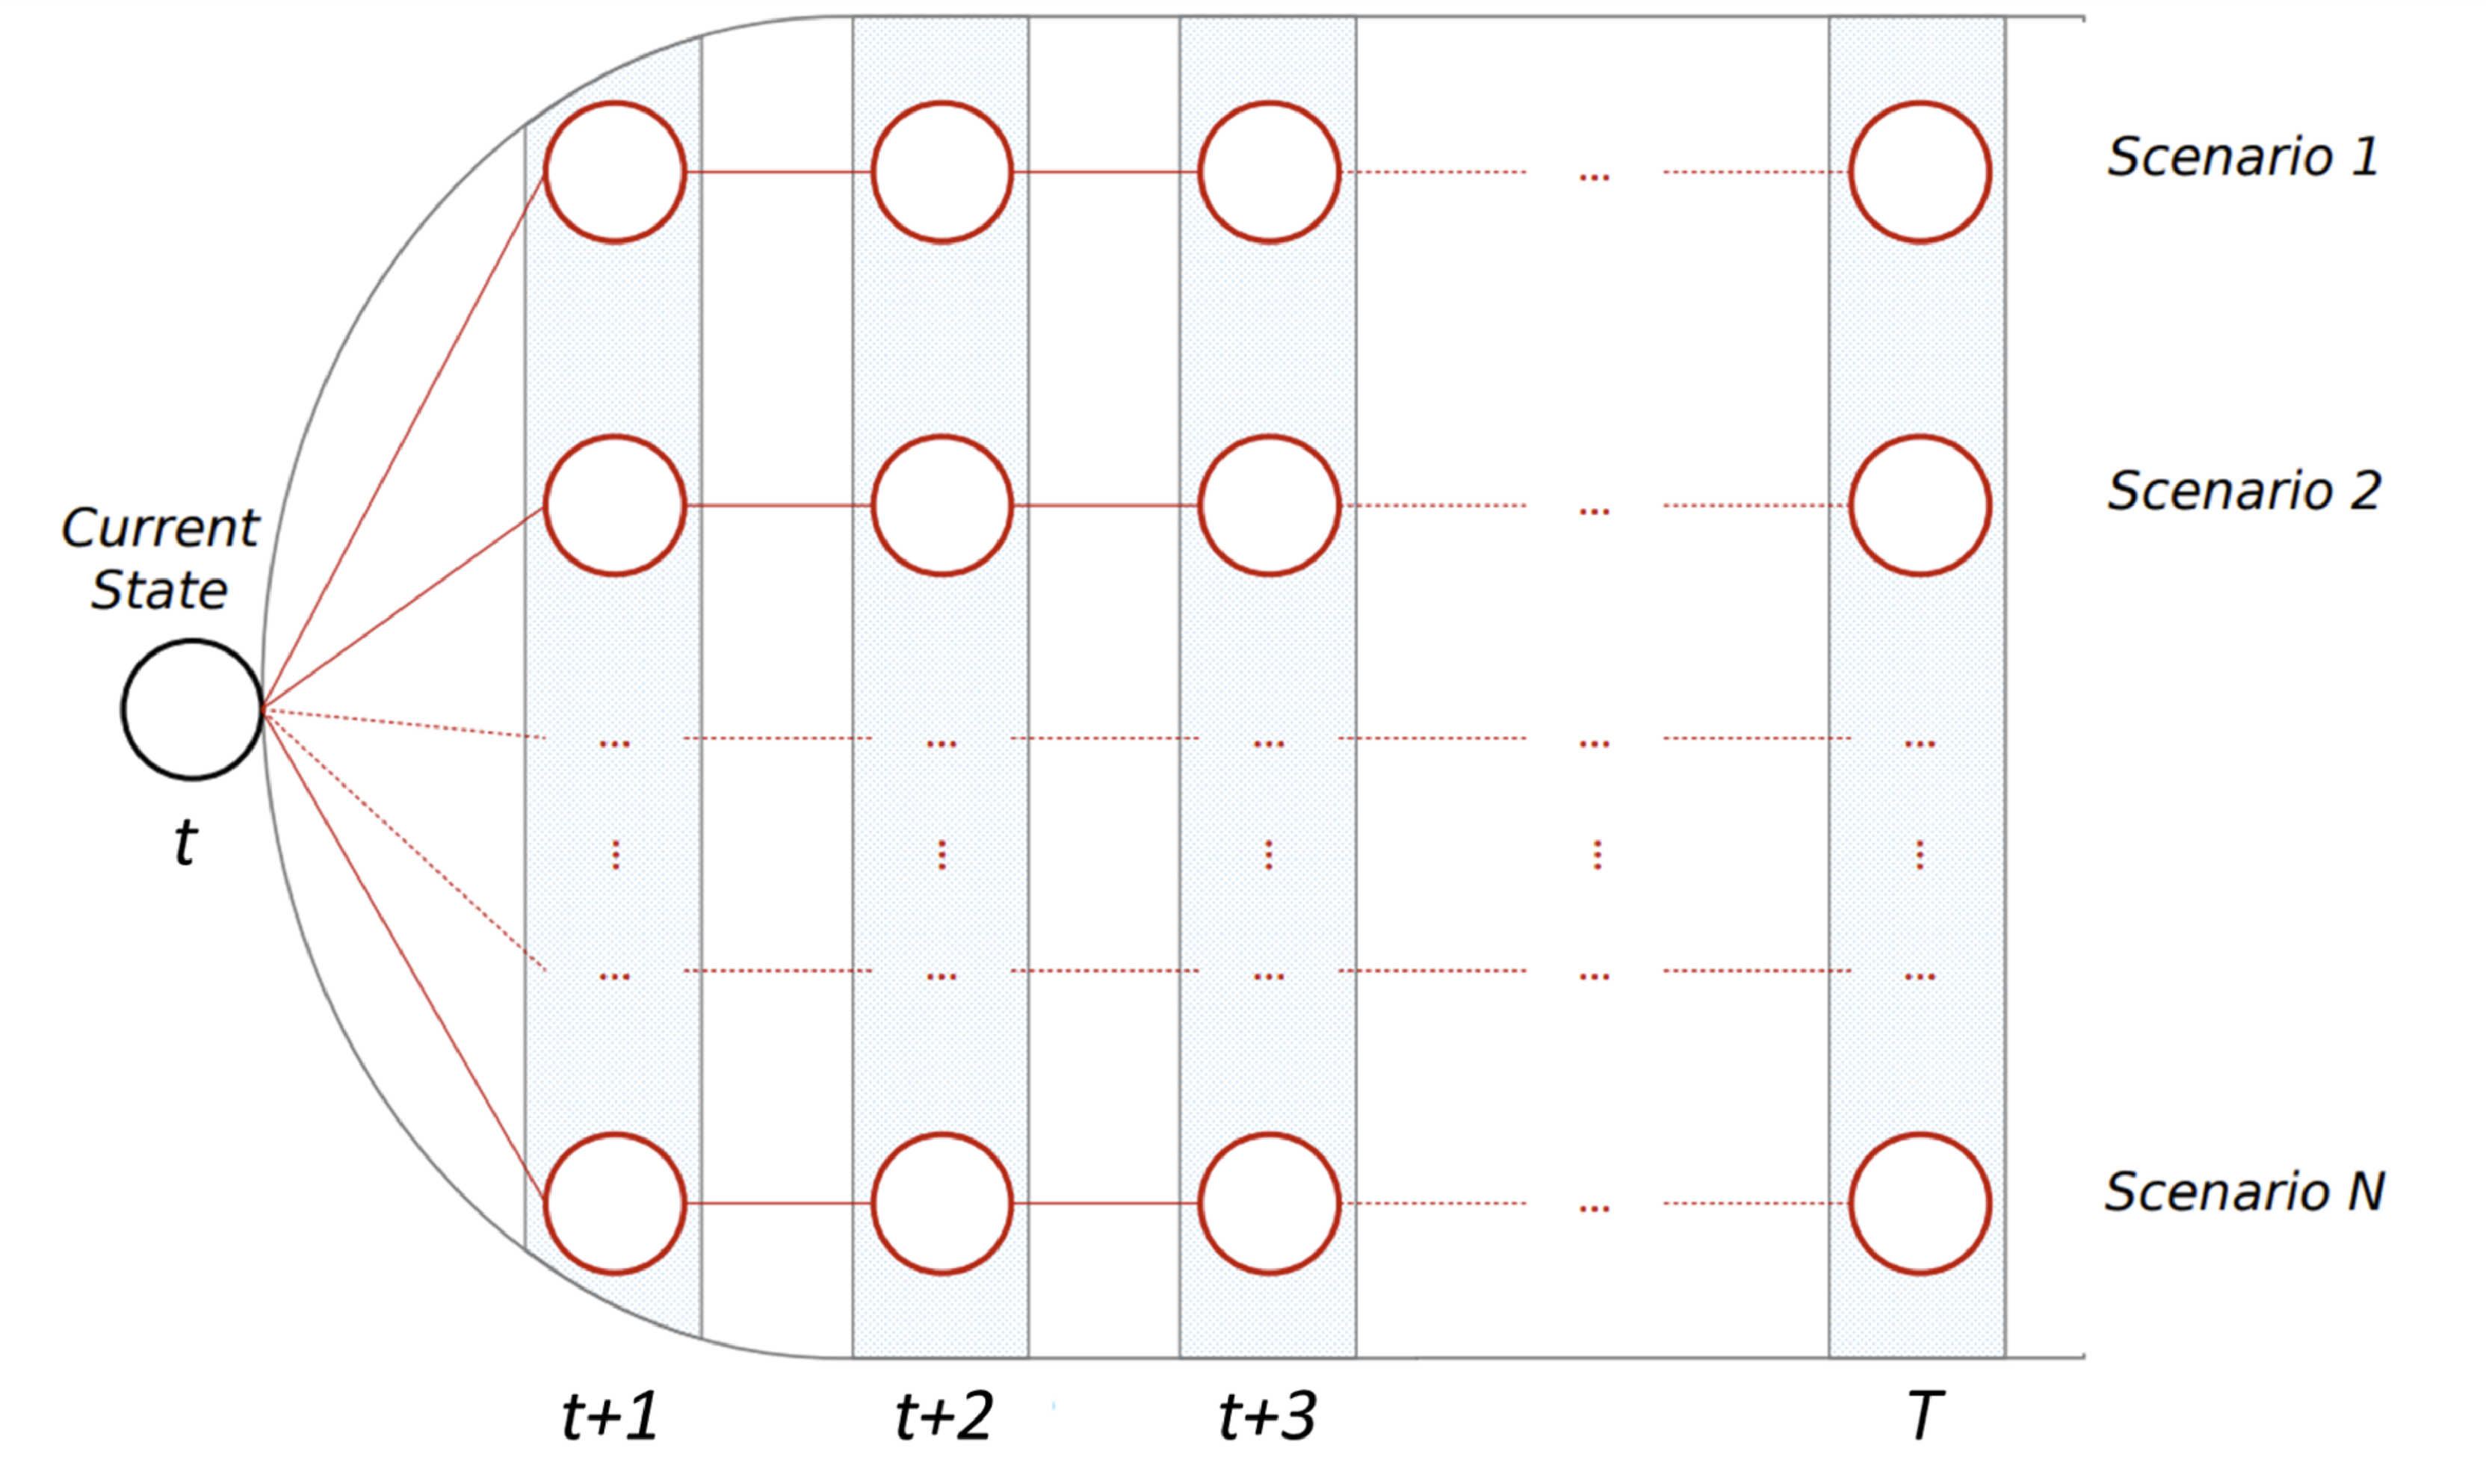
\includegraphics[width=0.65\textwidth]{scenarioExplained.pdf}
    \caption{Two-stage stochastic program built from $N$ level 2 scenarios. These are solved to find an implementable decision for stage \textcolor{red}{$t$} in a level 1 scenario.}
    \label{fig:explorations stochastic program}
\end{figure}

Given that stochastic programs are built for every state in every level 1 scenario, \textcolor{red}{the idea is to} approximate the continuous sample space of the exogenous variable from each state. \textcolor{red}{The higher number of level 2 scenarios $N$ the more accurate this approximation will be}. This approximation is illustrated in Figure \ref{fig:RSP state space}. The main difference compared to RI is that STRO makes multiple explorations (level 2 scenarios) from every state in every underlying level 1 scenario and uses these to approximate the sample space from that point. 
The red nodes in the figure represent the level 2 scenarios. New information about the underlying level 1 scenario is revealed with each step of the horizon. Thus, new two-stage stochastic programs must be built for every \textcolor{red}{state}  by generating new level 2 scenarios. 

None of the decisions made by STRO's heuristic are based on any knowledge of the future in the underlying price-inflow scenario. Following this, \textcolor{red}{the decisions made using the heuristic are implementable and} the value of the feasible policies found for every individual level 1 scenario yields lower bounds for the optimal revenue for that given scenario. Same as for RI, this means that with enough sampled scenarios, one will get an estimated lower bound of the expected revenue, subject to sampling error.
\begin{figure}[H]
    \centering
    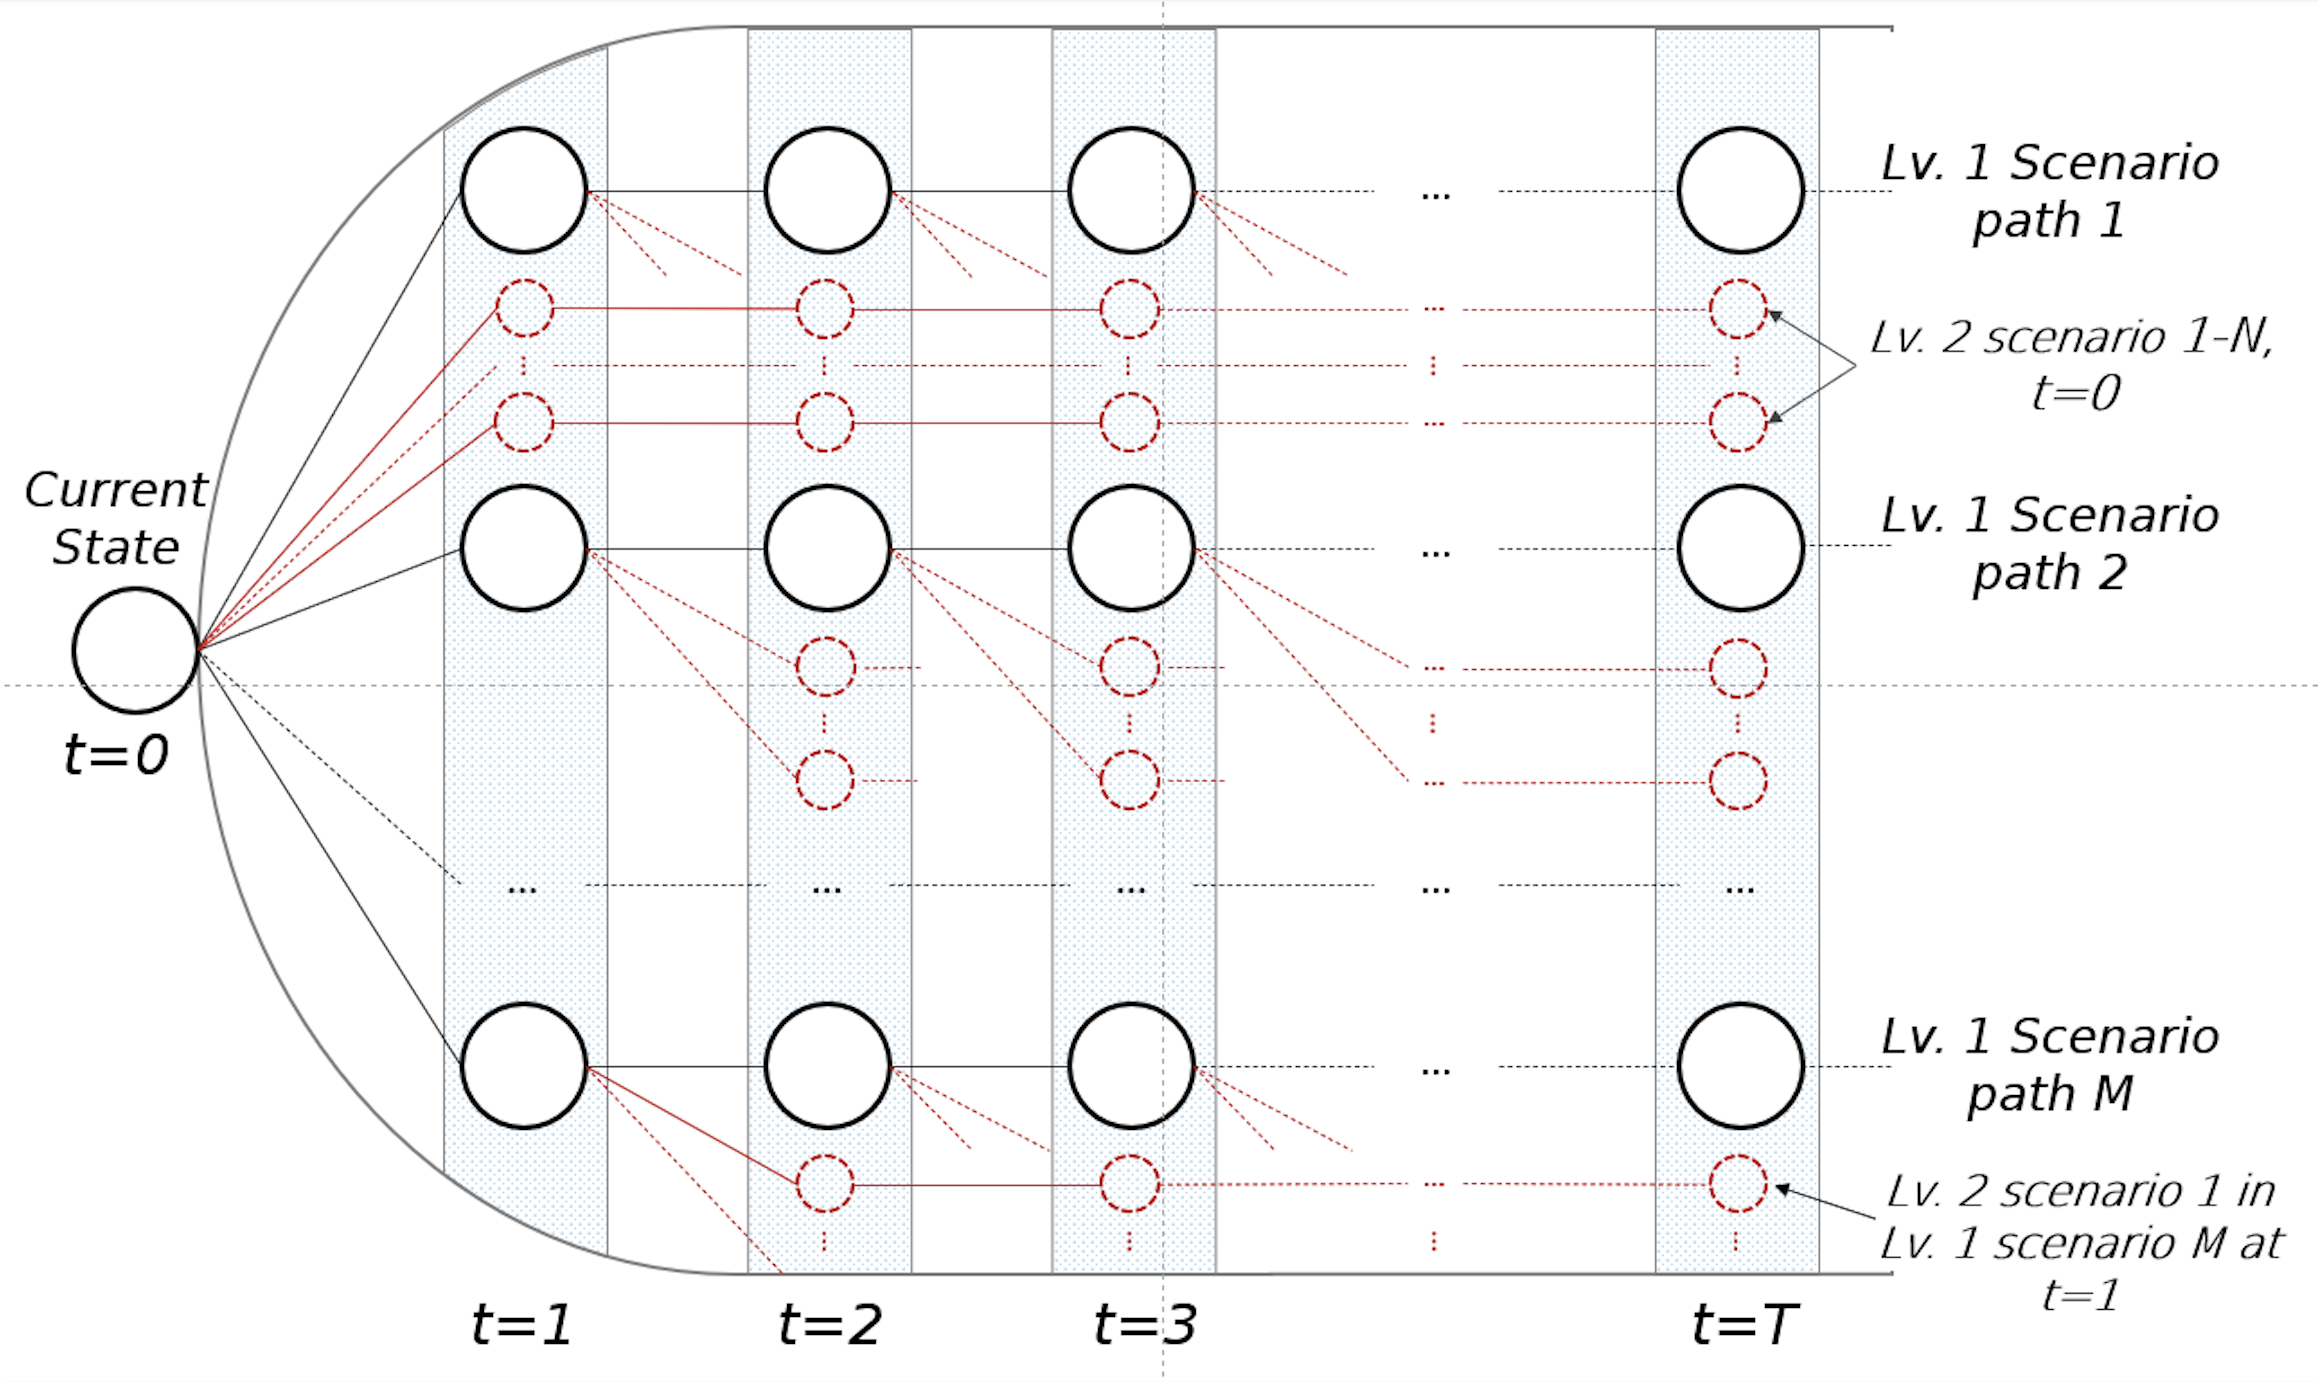
\includegraphics[width=0.8\textwidth]{discretizeRSP.png}
    \caption{Sample space approximation for STRO with  $N$ level 2 scenarios per \textcolor{red}{state} }
    \label{fig:RSP state space}
\end{figure}

As every generated level 2 scenario represents possible realizations of the sample space, one would gradually get a better approximation of all possible realizations of the future in all possible states by generating more scenarios per \textcolor{red}{state}.

As mentioned, the STRO heuristic finds the first-stage decision by considering these realizations as a two-stage program. Using two stages is an approximation, and a more accurate method would be to solve a multistage problem instead. However, building and solving multistage stochastic programs is more computationally costly, and approximation through two stages has been shown to be a good solution for hydropower problems in the literature \cite{SeAC17}. 

Due to the growth in complexity when increasing the number of level 2 scenarios per \textcolor{red}{state} , one can in practice only build programs based on a small number of scenarios. Therefore, the performance of STRO hinges on the assumption that most of the value from the approach can be achieved using a small number $N$ of level 2 scenarios, e.g.\ $N=2$ or $N=3$, which from early experiments seems to be the case.

\textcolor{red}{
\section*{Complexity}
Considering that the STRO heuristic is based on solving a two-stage stochastic program for every production decision, the amount of programs solved is quite large. Given $S$ level 1 scenarios and $T$ stages per level 1 scenario, one will have to solve a total of $ S \cdot T$ LPs to get an estimate of the marginal water value. 
}

\textcolor{red}{
Note that the number of LPs solved is not dependent on the amount of level 2 scenarios $N$. However, this instead affects the complexity of each LP, meaning that adding more level 2 scenarios makes the individual LP harder to solve.  
}

\section*{Main innovations and benefits}
As mentioned in \ref{section: problem description}, medium-term hydropower planning is mainly concerned with calculating the expected discounted revenue, given different initial water levels, to calculate the marginal value of the water in the reservoir. Consequently, there is no requirement to generate an implementable policy that deterministically yields the same production decision when faced with the same state, such as RI and SDDP. Instead, we relax this requirement and allow the STRO heuristic to yield stochastic production decisions based on the level 2 scenarios drawn from the sample space. We refer to this as policy relaxation. The benefit is that by not having to aggregate the possible outcomes, for instance, by taking the expectation such as RI, we can explore more of the sample space and consider more varied outcomes. As shown in the illustrative example in section \ref{section: illustrative example}, this can lead to more accurate revenue estimations. 

Another significant benefit of STRO and other rolling horizon methods is that they pose few constraints on the problem class. Unlike SDDP, which either requires inflow and price to be modelled linearly or with a Markov decision process over discretized states, this allows price and inflow to be modelled using non-linear methods such as deep learning-based methods. There is also no strict constraint that requires the problem to be modelled convexly, meaning that one for instance, could model head variations more accurately without having to relax the problem with McCormick envelopes. However, a non-convex model would require a longer processing time.  

Other significant benefits of rolling horizon methods such as STRO and RI is that they are significantly more straightforward to implement than SDDP and are more suited for parallelization since the level 1 scenarios are all solved independently. Although SDDP is also parallelizable, it is harder to implement and does not lead to as linear of a speedup\textcolor{red}{, as seen in previous works.}
 \textcolor{red}{One example is \cite{AvPL21} which reports speedup factors of 7--10 for 10 CPUs, and 9--14 for 20 CPUs, for a case study of the Brazilian hydrothermal system. Using a more detailed representation of the Brazilian power system, \cite{MaDB21} report speedup factors of 5--6.5 for 10  CPUs and 8--11 for 20 CPUs.}

We leave to further work to explore the practical merits of these benefits and concentrate our experiments on a case where SDDP can be used as a benchmark.




\section{Illustrative example}
\label{section: illustrative example}
This section illustrates the proposed heuristic using a simple three-stage example. Consider a plant operator with a current reservoir volume of 8, maximum reservoir capacity of 10, and maximum generation capacity of 10. In this setting, the chronology is as follows: First, inflow realizes, then the reservoir volume gets updated. Spillage happens if the current reservoir level plus inflowing water exceeds the reservoir capacity. Then the generation decision is taken before the new inflow arrives. 

The price is deterministic and given by $P_0 = 10, \ P_1 = 11, \ P_2 = 12$, incentivizing later production. Inflow is stochastic and the different scenarios can be seen in Figure \ref{fig: instance}. From every state, there is an equal chance that the subsequent inflow is high or low compared to the previous inflow. This results in a binary tree and 4 different scenarios since inflow is deterministic in the first stage. 

 \begin{figure}[H]
    \centering
    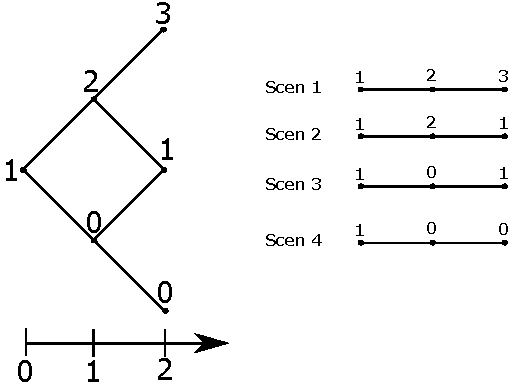
\includegraphics[width=0.6\textwidth]{RH_instance.pdf}
    \caption{Illustrative example inflow tree.}
    \label{fig: instance}
\end{figure} 

As an example: Since the current reservoir volume is 8 and 1 unit of inflow arrives deterministically, no spillage happens, as the reservoir can hold 10 units of water, allowing all units to be used for later generation. Suppose the producer decides to generate nothing at $t=0$, and the high inflow is realized at $t=1$ (scenario 1 or 2). In that case, 2 units arrive in addition to the 9 already in the reservoir, resulting in 1 unit of spillage.   

To see how RI and STRO with different numbers of level 2 scenarios perform for this example, we compare their different decisions and revenues in Table \ref{tab:sols}. We also compare them to the optimal strategy. Here we use $x_{i,j}$ to denote the production decision at time $i$ and state $j$, numbered according to the scenarios in Figure \ref{fig: instance}. The scenario index for stage 0 is omitted, as all these decisions need to be identical. \textcolor{red}{Similarly, in stage 1, we only use scenario indices $\{1,3\}$ since there only are 2 possible inflow realizations at $t=1$. Index 3 is used to stay consistent with the indices in stage 2.}

We observe that it is optimal to produce 1 unit in stage 0 to avoid spillage in the future. Rolling intrinsic, which bases decisions on expectations of the stochastic variables, ignores that there is a $50\%$ chance of 2 units of inflow getting realized in the next stage and only considers the expected inflow, which is $\frac{0+2}{2}=1$, thereby deciding to produce 0 at $t=0$. 

The notation STRO(N) is used in the table to indicate that N level 2 scenarios are used per \textcolor{red}{state}  for the STRO heuristic. Since there are only 4 possible realizations of the future, we use a maximum N of 4. 
For STRO(1), STRO(2) and STRO(3) the production decision naturally depends on which of the 4 scenarios are sampled. Since we sample the scenarios without replacement, the number of combinations of level 2 scenarios is ${4 \choose N}$, which results in 4, 6, 4 and 1 combinations for $N=1, 2, 3$ and $4$ respectively. The production decisions in the first stage are given in the table for all different combinations of level 2 scenarios in curly brackets. To deal with uncertain production decisions, we list the production decisions in the first stage for each combination of level 2 scenarios for every STRO(N) in curly brackets. Since the production decision at $t=0$ is uncertain for $N=1$ and $N=2$, the next state is also uncertain (STRO(3) yields the same production decision at $t=0$ independent of the combination of level 2 scenarios). For this reason, the production decisions at $t=1$ and $t=2$ are not listed for these, as these decisions naturally will depend on the previous decision, which is not deterministic. This relates to the discussed idea of policy relaxation, meaning that STRO does not necessarily generate an implementable policy.




\begin{table}[H]
\centering
\begin{tabular}{c c c c c c c} 
 \hline
  & Optimal & Rolling intrinsic & STRO(1) & STRO(2) & STRO(3) & STRO(4)\\ [0.5ex] 
 \hline\hline
 $x_0$ & 1 & 0 & $\{0,0,1,1\}$ &$\{0,1,1,1,1,1\}$ & $\{1,1,1,1\}$ & $1$ \\ 
 \hline
 $x_{1,1}$ & 3 & 2 & - & -&3&3 \\ % 2 \\
 \hline
 \textcolor{red}{$x_{1,3}$} & 0 & 0 & - &-&3&0\\ %  0 \\
 \hline
 $x_{2,1}$ & 10 & 10 & - &-&10&10\\ % 10 \\
 \hline
 $x_{2,2}$ & 8 & 9 & - &-&8&8\\ % 9 \\
 \hline
 $x_{2,3}$ & 9 & 10 & - &-&9&9\\ % 9.5 \\
 \hline
 $x_{2,4}$ & 8 & 9 & - &-&8&8\\% 8.5 \\
 \hline
 Mean spill & 0 & $\frac{3}{4}$ & $\frac{1}{2}$ & $\frac{1}{12}$ &0&0 \\
 \hline
 Mean profit & 131.5 & 125.0 & 127.0 & 130.83 & 131.5 & 131.5\\ [1ex] 
 \hline
\end{tabular}
\caption{Solutions and objective values. Note that STRO does not yield an implementable policy since there are several decisions at the first stage.}
\label{tab:sols}
\end{table}

The table shows that STRO(4) and STRO(3) both find the optimal strategy. This is unsurprising for STRO(4) as it considers all 4 possible scenarios when making decisions. STRO(3) does not have this privilege, but since it only omits a single possible level 2 scenario at $t=0$, it will always sample at least one of the 2 scenarios with \textcolor{red}{high} inflow at $t=1$. This allows it to see that there is a chance of spillage occurring and thereby plan its production accordingly.

It can further be seen that STRO(1) and STRO(2) both outperform RI, despite not necessarily seeing that there is a chance of high inflow at $t=1$. As STRO(2) will sample 2 level 2 scenarios per \textcolor{red}{state} it will not consider the chance of high inflow only in the case that the 2 level 2 scenarios are both low inflow scenarios. There is only a $\frac{1}{6}$ chance that this happens, making it unlikely that the wrong production decision is made. When making a decision at $t=1$ there are only 2 possible future inflow realizations, depending on the previously observed inflow. As a consequence of this, STRO(2) will make the optimal decisions at $t=1$ since it can consider both possible future realizations from that point. 

STRO(1) only samples a single level 2 scenario \textcolor{red}{per state}  At $t=0$ it is only a $50\%$ chance that it samples a high inflow scenario and adjusts production to avoid risking spillage. However, it still outperforms RI, because RI will only consider the expected inflow of 1, meaning that it will always make the wrong production decision at $t=0$. The same effect would be seen if a high inflow scenario was realized at $t=1$. Then RI would not take the fact that a high inflow of 3 could occur at $t=2$ into account and only consider the expected inflow of $2$. This results in a higher chance of spillage. 

\textcolor{red}{Although STRO(1) outperforms RI in this illustrative example, it must be stressed that this is not the case in general, and under different circumstances RI has been found to outperform the simplest version of STRO, as we will demonstrate in the next section.}
%\clearpage